\documentclass{article}
\usepackage[margin=0.625in]{geometry}
\usepackage{parskip, setspace}
\setstretch{1.15}
\usepackage{amsmath, amsfonts}
%\numberwithin{equation}{subsection}
\usepackage{graphicx, caption}
\usepackage{hyperref}
\usepackage[ruled, linesnumbered, noend]{algorithm2e}
\usepackage[english]{babel}

\title{\vspace{-0.625in}CS 529: Advanced Data Structures \& Algorithms \\ Assignment 1}
\author{Nathan Chapman, Hunter Lawrence, Andrew Struthers}
\date{\today}

\begin{document}
\maketitle

\section*{Creating a 3-2 Tree}

    A binary search tree (BST) is usually an excellent choice of data structure because inserting, deleting, and searching all take $O(n)$.  This linear complexity arises because the tree can be ``completely'' unbalanced, yielding a linear search.  B-Trees circumvent this by rebalancing upon each insertion and deletion.

    An example of how the re-balancing is implemented for B-Trees can be shown in the context of the simplest B-Tree: the 3-2 tree.  The following algorithms implement insertion, traversal and ``bumping and breaking'' of the nodes of a 3-2 tree.

    \subsection*{Recursive Implementation}

        \subsubsection*{Algorithm}

            The core functionality of what differentiates a B-tree from a BST (i.e. the automatic rebalancing) is encapsulated in \texttt{bumpAndBreak}.

            \begin{function}
                \caption{bumpAndBreak(p)}
                \DontPrintSemicolon

                \KwIn{node $p$}
                \KwOut{Null}

                \eIf{p has a parent}{
                    insert $p.keys[2]$ into $p.parent.keys$
                }{
                    create parent node with key $p.keys[2]$\;
                }
                remove $p.keys[2]$\;
                create $parent.left$ with key $min \ p.keys$\;
                create $parent.right$ with key $max \ p.keys$\;
                remove $parent.middle$\;
            \end{function}

            We can use \texttt{bumpAndBreak} upon recursively traversing down to a leaf that, after insertion of the a new key, has 3 keys.

            \begin{function}
                \caption{insertRecursive(p, k)}
                \DontPrintSemicolon

                \KwIn{node $p$, new key $k$}
                \KwOut{3-2 B-tree}

                \If{$p$ is a leaf}{
                    insert $k$ into $p.keys$\;
                    sort $p.keys$\;
                    \If{length of p.keys = 3}{
                        bumpAndBreak(p)
                    }
                }
                \ElseIf{$k < p.keys[1]$}{
                    \insertRecursive(p.left, k)\;
                }
                \ElseIf{$k > p.keys[end]$}{
                    \insertRecursive(p.right, k)\;
                }
                \Else{
                    \insertRecursive(p.middle, k)\;
                }
            \end{function}
        
    \pagebreak

            Finally, we can exectute the above algorithms for each element in a list of keys to create a 3-2 B-Tree.

            \begin{function}
                \caption{buildTree(keyList)}
                \DontPrintSemicolon

                \KwIn{List of keys}
                \KwOut{3-2 Tree of given keys}

                create root node with key $keyList[1]$\;

                \ForEach{$key \in keyList[2:end]$}{
                    insertRecursive(root, key)
                }
            \end{function}

        \subsubsection*{Complexity}

            To analyze the complexity of this algorithm, each sub-algorithm can be inspected and their complexities multiplied.  We first start with the top most algorithm \texttt{buildTree}, and follow the stack trace down to \texttt{bumpAndBreak}.

            Because \texttt{buildTree} must be called for every element in the input list of length $n$, its complexity is $O(n)$.  Then for each element in the input list, we must recursively traverse the tree until reaching the point at which the new key will be in a sorted position; as with all binary trees, this takes $O(\lg(n))$ time.  Finally, the operations in \texttt{bumpAndBreak} are only ever on a single input and thus the total number does not scale with the size of the input.

            In total, we combine each of these to acheive a runtime complexity of $O(n \lg (n))$ of using this algorithm to create a 3-2 B-tree from a list of $n$ keys.

    \subsection*{Iterative Implementation}

We also wrote an interative version of the 3-2 Tree construction, seen below. For each key in the keys list, we call function \texttt{insertKey} with a reference to the head node of the tree and the key we want to insert. The algorithm then traverse iteratively down the tree from the head, finding the leaf where the key should be inserted. Once that leaf is found, insert the key into that leaf's keys, preserving the sorted order of the keys. Then, the algorithm handles the possible case where there are 3 keys in a node, by breaking up the current node into a left and right node, whose children and keys are assigned from the current node. The middle key gets inserted into the current node's parent, and then sets the current to the current node's parent. This process is repeated until the current node no longer has 3 keys. The tree grows at the root level, so all leaves are preserved at the bottom of the tree.

\texttt{traverseTree} runs in $O(\text{log}n)$ time, because the algorithm traverses depth first into a tree structure. The traversal skips all invalid nodes by only moving to the appropriate child. \texttt{handleKeyOverflow} also runs in $O(\text{log}n)$ time, since it traverses the tree from a single leaf up to the root node, which takes the same runtime as traversing from the root node to a single leaf. \texttt{breakNode} runs in constant time. Therefore, the insertion of a key into the 3-2 tree structure using an iterative algorithm is $O(\text{log}n)$ time, which matches the expected insertion operation time.

\begin{function}
	\caption{insertKey(head, key)}
	\DontPrintSemicolon
	\KwIn{Head node of tree $head$, key to be inserted $key$}
	$current$ $\gets$ \texttt{traverseHead}($head$, $key$)\;
	insert key into $current$ keys\;
	\texttt{handleKeyOverflow}(current)\;
\end{function}

\begin{function}
	\caption{traverseTree(head, key)}
	\DontPrintSemicolon
	\KwIn{Head node of the tree $head$, key to be inserted $key$}
	\KwOut{Leaf node where $key$ should be inserted}
	$current$ $\gets$ $head$\;
	\While{current node is not a leaf}
	{
		\If{key $\leq$ current first key}
		{
			$current$ $\gets$ $current$ left child\;
		}
		\ElseIf{key $\geq$ current first key}
		{
			$current$ $\gets$ $current$ right child\;
		}
		\Else
		{
			$current$ $\gets$ $current$ middle child\;
		}
	}
\end{function}

\begin{function}
	\caption{handleKeyOverflow(current)}
	\DontPrintSemicolon
	\KwIn{Current node in the tree $current$}
	\While{number of keys in $current$ $=$ 3}
	{
		$middle\_key$ $\gets$ middle key of node\;
		\If{$current$ parent node is null}
		{
			create new parent node\;
			$current.parent$ $\gets$ to new node\;
		}
		insert $middle\_key$ to parent node\;
		create new $left\_node$ and $right\_node$\;
		\texttt{breakNode}($current$, $left\_node$, $right\_node$)\;
		delete $middle\_key$ from $current$ keys\;
		$left.parent$ $\gets$ $current.parent$\;
		$right.parent$ $\gets$ $current.parent$\;
		$current$ $\gets$ $current.parent$\;
		delete old $current$\;
	}
\end{function}

\begin{function}
	\caption{breakNode($current$, out $left$, out $right$)}
	\DontPrintSemicolon
	\KwIn{Current node in tree $current$, new left node $left$, new right node $right$}
	\KwOut{Constructed $left$ and $right$ nodes as out parameters}
	$left$ $\gets$ parent to $current$ parent\;
	$right$ $\gets$ parent to $current$ parent\;
	insert first key from $current$ to $left$\;
	insert last key from $current$ to $right$\;
	\If{$current$ is not a leaf}
	{
		insert two left children from $current$ as $left$ children\;
		insert two right children from $current$ as $right$ children\;
	}
\end{function}

\vspace{1in}

\section*{Discussion on van Emde Boas Trees}

Van Emde Boas (vEB) Trees are a data structure which stores a fixed number of ${M = 2^m}$ binary vectors in an index addressable array. Each index in this array represents the presence (1) or absence (0) of that element in the structure. From this list, it creates and stores a summary vector tree containing binary values identifying the presence of a positive bit within its vector. An example of a vEB tree of order 16 can be seen below.

\begin{figure}[h]
    \centering
    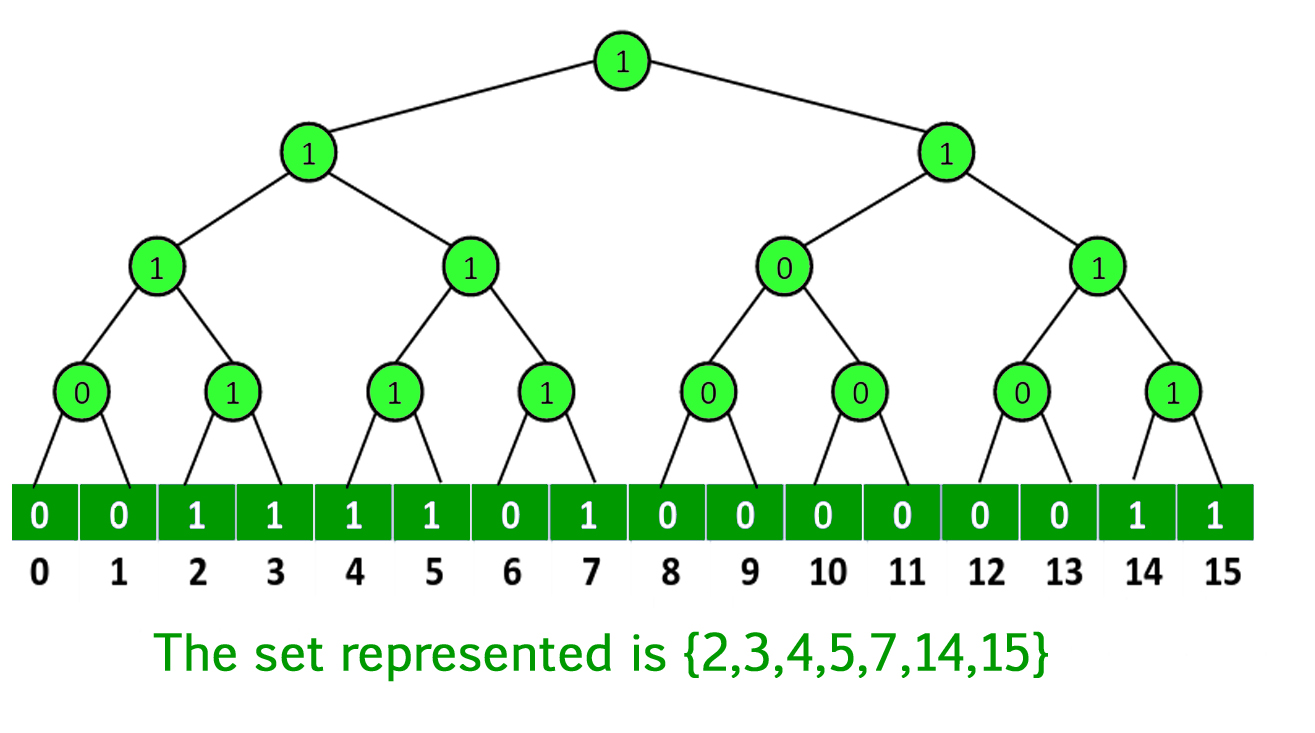
\includegraphics[width=\textwidth,keepaspectratio]{Images/vEB_tree_GFG.jpg}
    \label{fig: vEB}
    \caption{An example proto van Emde Boas Tree from GeeksForGeeks.org}
\end{figure}

Unlike other structures, the index addressable nature of the structure vEB trees are buit on allows for location, insertion, and deletion operations to be performed in constant $O(\text{1})$ time simply by changing the bit at the index representing the value in the tree, then updating the summary vector. The major strength of vEB trees over other structures is how it can handle locating the next positive value from any given value in $O(\text{log log} M)$ time.

An example use case for vEB trees might include the location of the next nearest empty parking space. Assuming that 1) the car is near a parking space that is already taken, 2) that the spaces are ordered in a way that represents distance from one another (i.e. space \#3 is closer to space \#5 than space \#6), and 3) that a 1 will represent an empty parking space. After locating the current spot in constant time, the ability of vEB trees to find a successor or predecessor of an empty spot in $O(\text{log log } M)$ time might prove useful.

Unfortunately, the limitations of vEB trees make other algorithms (such as Skip Lists) much more preferable for solving successor and predecessor problems. While the constant time insertion and deletion are ideal, the limitation that they may only represent integer values is a major limitation. The fixed size also restricts what the structure can be allowed to represent, since the data may only be dynamic within a certain range. And finally, the fixed space requirement of $O(\text{M})$ makes the structure cumbersome. These drawbacks, combined with the fact that structures like Skip Lists can perform next nearest neighbor functions on more versatile objects in $O(\text{log} n)$ time, makes them more useful over vEB trees.

\pagebreak

\section*{Discussion on Skip Lists}

Skip lists are an extension on the standard linked list. This data structure on average preserves the space efficiency of a linked list, but due to the random nature of this structure, could have worst case $O(n \text{log} n)$ space efficiency. Skip lists also have the insertion/deletion ease of a linked list, where each node in the list has a pointer to the next (and sometimes previous) node, while also benefiting from the searching speed of various tree structures. This data structure is a randomized data structure, and it allows an average complexity of $O(\text{log} n)$ for insertion and searching. This means that on average, a skip list has the best features of a sorted array, capable of random memory access while searching, while maintaining the linked list structure, meaning that insertion requires very low time complexity. 

A skip list can be thought of as a layered linked list. The bottom layer is denoted as $L(0)$, and then higher layers are denoted as $L(1)$, $L(2)$, \ldots, $L(n)$. An element of the skip list has a $\frac{1}{2^m}$\% chance of being on layer m. If an element appears on layer m, the element also must appear on layer $m-1$, $m-2$, \ldots, $0$. An image of a skip list can be seen below

\begin{figure}[h]
    \centering
    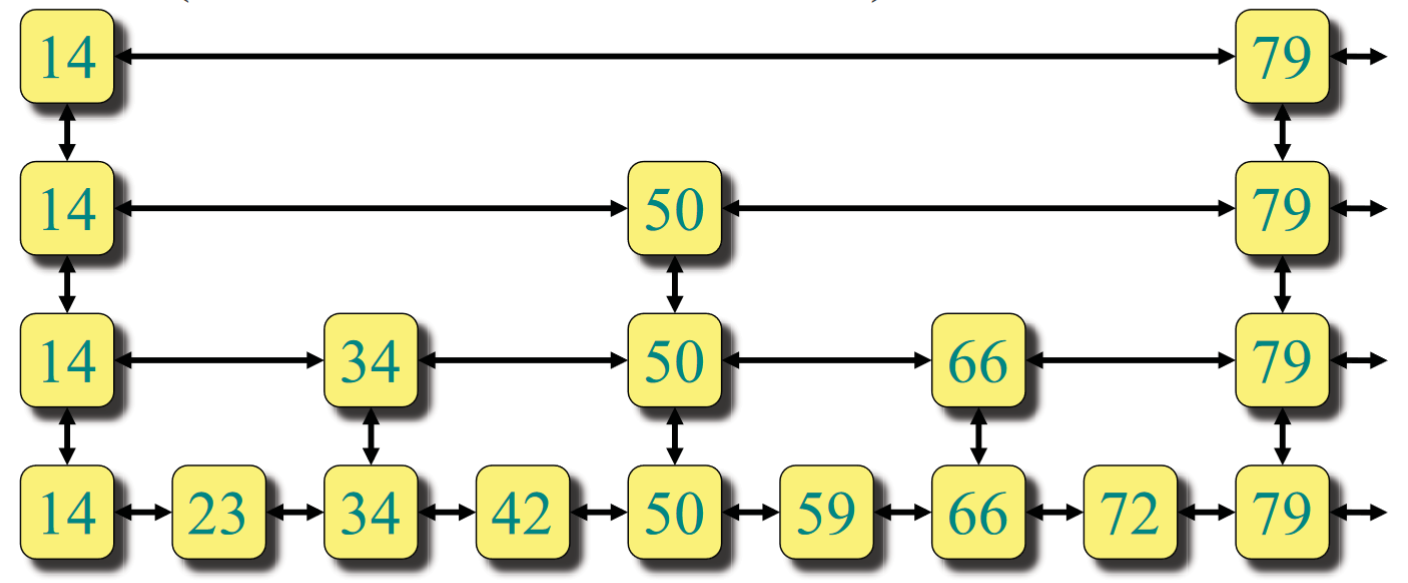
\includegraphics[width=\textwidth,keepaspectratio]{Images/SkipList_MIT.PNG}
    \label{fig:skip_list}
    \caption{An example of a skip list from the MIT lecture slides}
\end{figure}

The hierarchical structure of the layers results in an average time complexity of $O(\text{log} n)$ for search, insert, and delete operations and a worst case of $O(n)$. This structure uses randomness and a layered linked list to skip over portions of the data when performing search operations, to a very similar effect as a binary search tree. The linked list structure is more beneficial than a binary search tree, however, because there is no need to rebalance the tree after every insertion or deletion with a skip list.

A common real-world representation of a skip list is buses in a busy city. In downtown Seattle, for example, there are many bus stops. Some buses go from stop to stop, whereas some buses stop at one high traffic stop, then cross town, skipping many lower traffic stops in the process. This is the same idea as a skip list, where the bottom row is analogous to the bus that stops at every destination, and the higher up rows in the skip list hierarchy are analogous to the buses that take people from one high traffic destination to another, skipping over some stops. 

Skip lists have many applications, especially in high traffic operations where rebalancing a tree or linearly searching through a massive array would take too long. One of the common applications of skip lists in industry is using this data structure as a way to index databases and database tables. Another application of skip lists is in priority queues, where one specific example could be CPU job scheduling. CPU job scheduling is a very time-sensitive process, where jobs could be swapped out many times per second. Maintaining a priority queue with a skip list, where each node in the list is a priority of a job, allows the priority queue to operate in logarithmic time, where insertion and deletion is much faster than a standard queue implementation, and a tree structure doesn’t need to be constantly maintained and rebalanced as jobs get added to or removed from the system.



\pagebreak

\end{document}